\documentclass[12pt,
    a4paper,
    headinclude,
    footinclude]{scrreprt}

    %plainfootsepline

\usepackage{blindtext}
\usepackage[utf8]{inputenc}
\usepackage{setspace}
\usepackage[ngerman]{babel}
\usepackage[ngerman, num]{isodate}
\usepackage[left=3cm,right=2cm,top=2.8cm,bottom=1.6cm]{geometry}

\usepackage[style=numeric]{biblatex}
\usepackage[babel,german=guillemets]{csquotes}

\usepackage{float}

\usepackage{graphicx}

\usepackage{listings}
\usepackage{color}
\renewcommand{\lstlistingname}{Auflistung}
\renewcommand{\lstlistlistingname}{Auflistungsverzeichnis}
\definecolor{hellgrau}{rgb}{.95,.95,.95}
\definecolor{grau}{rgb}{.9,.9,.9}
\lstset{
	%backgroundcolor=\color{hellgrau},
	%backgroundcolor=\color{blue}
	%basicstyle=\scriptsize\ttfamily,
	%keywordstyle=\bfseries\ttfamily\color{orange},
	%stringstyle=\color{green}\ttfamily,
	%commentstyle=\color{middlegray}\ttfamily,
	%emph={square}, 
	%emphstyle=\color{blue}\texttt,
	%emph={[2]root,base},
	%emphstyle={[2]\color{yac}\texttt},
	showstringspaces=false,
	%flexiblecolumns=false,
	tabsize=1,
	numbers=left,
	%numberstyle=\tiny,
	numberblanklines=false,
	stepnumber=1,
	%numbersep=0pt,
	xleftmargin=20pt,
	frame=l,
	framesep=4.5mm,
	framexleftmargin=2.5mm,
	fillcolor=\color{grau},
	rulecolor=\color{grau},
	%numberstyle=\normalfont\tiny\color{numbercolor}
}

\usepackage{wrapfig}

\bibliography{res33.bib} 


\AtBeginDocument{\setlength{\glslistdottedwidth}{.15\columnwidth}}
\usepackage[acronyms,style=listdotted,shortcuts,translate=babel,toc]{glossaries}
%\GlsSetXdyLanguage{german}                         % Deutsche Spracheinstellung (nicht ngerman!) 
%\GlsSetXdyCodePage{duden-utf8}                     % Deutsche Codierung 
%\newglossarystyle{glosstil}{                     % neuer Stil mit Namen
%	\glossarystyle{listdotted}                           % basierent auf Stil long
%	\renewenvironment{theglossary}
%	{\begin{longtable}
%			{@{}p{0.1\textwidth} p{0.8\textwidth}}}   % einstellen der Spaltenbreiten
%		{\end{longtable}}
%	\renewcommand*{\glsgroupskip}{}               % keine Gruppenumbrüche
%} 

%\renewcommand*{\glsgroupskip}{}
%\makeglossaries
% \newacronym{TCP}{TCP}{Transmission Control Protocol}
% \newacronym{FTP}{FTP}{File Transfer Protocol}
% \newacronym{IP}{IP}{Internet Protocol}
% \newacronym{DNS}{DNS}{Domain Name Server}
% \newacronym{WWW}{WWW}{World Wide Web}
% \newacronym{HTTP}{HTTP}{Hypertex Transfer Protocol}
% \newacronym{HTTPS}{HTTPS}{Hypertex Transfer Protocol Secure}
% \newacronym{HTML}{HTML}{Hypertex Markup Language}
% \newacronym{XML}{XML}{Extensible Markup Language}
% \newacronym{WS}{WS}{WebSocket}
% \newacronym{ASCII}{ASCII}{American Standard Code for Information Interchange}
% \newacronym{UTF-8}{UTF-8}{8-Bit Universal Character Set Transformation Format}
%\usepackage{etoolbox}

%\newacronym{}{}{}

%\usepackage{fontspec}
%\setmainfont{Times New Roman}
%\usepackage[T1]{fontenc}
%\newcommand{\changefont}[3]{
%\fontfamily{#1} \fontseries{#2} \fontshape{#3} \selectfont}

%\renewcommand{\chapterpagestyle}{scrheadings}


%kopf und fusszeile
\usepackage[headsepline]{scrpage2}
\pagestyle{scrheadings} 
\setlength{\footskip}{8mm}
\clearscrheadings
\ihead{\leftmark}
\ohead{\rightmark}
\automark[section]{chapter}
\cfoot{\pagemark}
%kopf und fusszeile

%Schriftart sfffamily serifenlos
\setkomafont{pageheadfoot}{\normalfont\rmfamily\bfseries}

\setkomafont{chapterentry}{\normalfont\rmfamily\bfseries}
%\setkomafont{sectionentry}{\normalfont\rmfamily}

\setkomafont{chapter}{\huge\normalfont\rmfamily\bfseries}
\setkomafont{section}{\Large\normalfont\rmfamily\bfseries}
%Schriftart



\DefineBibliographyStrings{ngerman}{%
	bibliography={Literaturverzeichnis}% NICHT references
}


\author{Martin Braun}
\title{Redfish}

\begin{document}
	\onehalfspacing
	\monthyearsepgerman{\,}{\,}
	\setcounter{tocdepth}{2}
	

	
	\begin{titlepage}
	
		\begin{center}
			~\\[2cm]
			Berufsakademie Sachsen \\
			Staatliche Studienakadamie Leipzig \\[2.4cm]
           
			\begin{huge}
			    \textbf{Binäre und reelle Codierung im Vergleich} \\[2.4cm]
			\end{huge}
			
			\doublespacing

			Evolutionäre Algorithmen 


		\end{center}
		
		\onehalfspacing
		\begin{tabbing}
			Eingereicht von: \= ~ \= ~ \= ~ \= Georg Andrassy \\
			\> \> \> \> Martin Braun \\
			\\

		\end{tabbing}
		\vspace*{\fill}
		Leipzig, \today
		
	\end{titlepage}
    
    %Inhaltsverzeichnis
    \pagenumbering{Roman}
%    \tableofcontents 	
    \clearpage
    %Inhaltsverzeichnis
        
    \pagenumbering{arabic}
    \setcounter{page}{2}
    
\section*{Einführung}	\onehalfspacing
	
.

.

.

.


	
	
\section*{Umsetzung}

	\begin{itemize}
	
	
	\item Zahl: Folge der Ziffern 0-9
	\item String: enthält eine Zeichenkette
	\item Array: geordnete Liste von Werten die mit  formatiert wird
	\item Objekt: eine ungeordnete Liste von Eigenschaften, bestehen aus einem Schlüssel und einem Wert (Schlüssel:Wert). Der Schlüssel ist String, der Wert kann ein Objekt, Array, eine Zahl, ein boolscher Ausdruck oder wiederum ein String sein. 
	\item Boolean: entweder true oder false
	\item Nullwert: mit Schlüsselwort null gekennzeichnet
	
	
\end{itemize}
	



	
\section*{Ergebnisse}	


		\begin{figure}[H]
			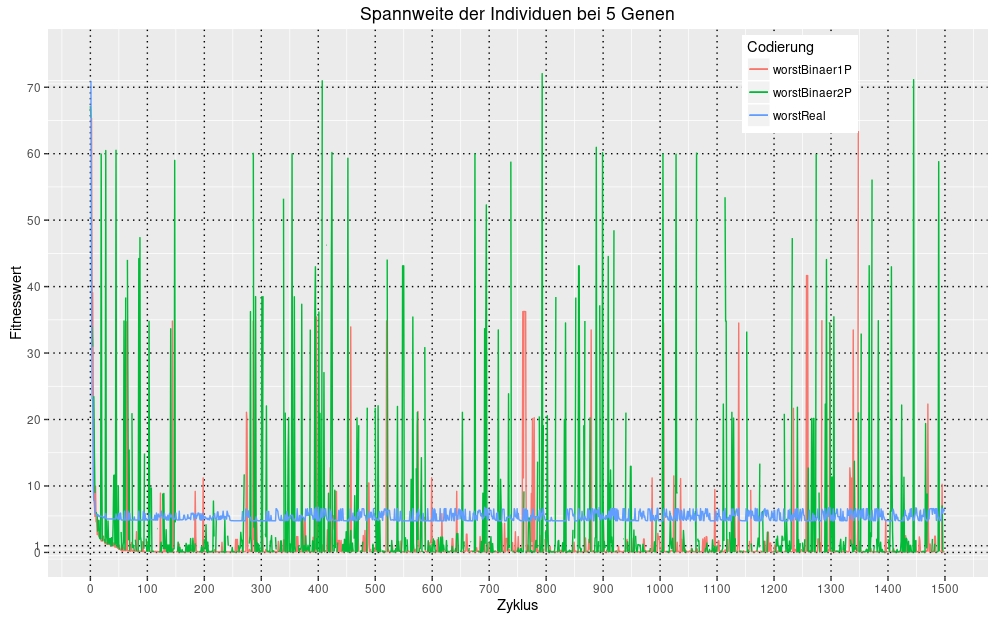
\includegraphics[width=0.95\textwidth]{spannweite-5-gene.jpeg} 
			
			\caption{Spannweite bei 5 Genen} 
			\label{InputOutput}
		\end{figure}

	
	

	

	
	

	

	


	

	
	
	



%	\glsnogroupskiptrue
%	\printglossary[type=\acronymtype, title=Abkürzungsverzeichnis]
	
%	\listoffigures
%	\addcontentsline{toc}{chapter}{Abbildungsverzeichnis}
	
%	\lstlistoflistings
%	\addcontentsline{toc}{chapter}{Auflistungsverzeichnis}
	
%	\printbibliography 
%	\addcontentsline{toc}{chapter}{Literaturverzeichnis}
	
	
	%\begin{acronym}
	%	\acro{TCP}{Transmission Control Protocol}
	%	\acro{FTP}{File Transfer Protocol}
	%	\acro{IP}{Internet Protocol}
	%	\acro{DNS}{Domain Name Server}
	%	\acro{WWW}{World Wide Web}
%	\end{acronym}

\end{document}